\documentclass[12pt,oneside]{report}
\usepackage[italian]{babel}
\usepackage[utf8]{inputenc}
\usepackage{graphicx}
\graphicspath{{images/}}
\usepackage{subcaption}
\usepackage[a4paper,top=25mm,bottom=25mm,bindingoffset=6mm,hmargin={3.5cm,3cm}]{geometry}
\usepackage{natbib}
\newtheorem{theorem}{Teorema}
\usepackage{mathtools}
\usepackage{amsmath}
\usepackage{amsfonts}
\usepackage{enumitem}
\usepackage{epsfig}
\usepackage{float}
\usepackage[bottom]{footmisc}
\linespread{1.5}
\usepackage{titlesec}
\titleformat{\chapter}[display]
{\normalfont\huge\bfseries}{}{0pt}{\Huge}
\titlespacing*{\chapter} {0pt}{20pt}{40pt}

\usepackage{minted}
\usemintedstyle{emacs}
\usepackage{xcolor}
\renewcommand{\theFancyVerbLine}{\sffamily \textcolor[rgb]{0,0,0}{\large \oldstylenums{\arabic{FancyVerbLine}}}}

\begin{document}

\begin{titlepage}
%\pagestyle{empty} 
\begin{center}
{\Large Università degli Studi di Salerno}\\[0.2truecm]
{\large Dipartimento di Informatica}\\
\hrulefill
\vfill

\epsfig{file=images/logoUnisa.jpg,width=5truecm}\\[0.2truecm]
\vfill

{\large Tesi di Laurea Triennale in }\\[0.2truecm]
{\Large Informatica}\\
\vfill\vfill
{\large QUERY RELAXATION GUIDATA DA DIPENDENZE FUNZIONALI APPROSSIMATE}
\vfill\vfill


 {\bf Relatore} \hfill {\bf Candidato}\ \ \\
Prof. Vincenzo Deufemia \hfill Domenico Antonio Tropeano \\
\hfill Matr. 0512102981
\vfill
\hrulefill 

Anno Accademico 2016-2017

\end{center}

\end{titlepage}
%\clearpage
%\setcounter{page}{1}
\chapter*{Abstract}
Negli ultimi anni la crescita delle reti ha portato ad un aumento del flusso di dati, si è reso così necessario uno sforzo maggiore per catalogare, indicizzare e pulire i  dati. 
La branca dell’informatica più inerente a questo problema è quella legata alle Basi di Dati. 
Quando si progetta un Database si tiene conto di alcuni importanti parametri che ne attestano la qualità, in particolare si cercano le dipendenze funzionali. Tali dipendenze vengono infatti utilizzate per per ridurre le anomalie e migliorare la qualità del Database.
Le dipendenze funzionali hanno però anche altri utilizzi, che si sono resi evidenti nell’ultima decade. Dato che all’aumento della quantità di dati verificatosi negli ultimi anni è conseguito un aumento inversamente proporzionale della qualità,è stato necessario  adattare le dipendenze funzionali per individuare le inconsistenze in modo più ampio.
Le Dipendenze funzionali rilassate o approssimate (RFD) sono una generalizzazione delle dipendenze funzionali canoniche, possiedono delle caratteristiche che le rendono più adattabili, infatti la dipendenza può applicarsi solo ad alcune tuple e non a tutto il Database e cosa più importante il concetto di uguaglianza delle FD viene sostituito nelle RFD  con il concetto di similarità. 
Il lavoro di tesi è consistito nell’utilizzare le RFD in un sistema di Query Relaxation che permette di ottenere un Result Set più ampio nel caso in cui il risultato di una query non sia soddisfacente.
Il concetto ivi sviluppato non riguarda il semplice ampliamento dei range sui vincoli di una query, bensì grazie alle RFD  è possibile modificare/sostituire i vincoli della query ottenendo un Result Set più ampio che sia però in qualche modo correlato al Result Set iniziale.
\tableofcontents
\listoftables
\renewcommand\listoflistingscaption{Elenco degli snippet di codice}
\listoflistings

\chapter*{Dedica}

\chapter{Introduzione}
\section{Incipit}

In un modello relazionale, la scoperta dipendenza funzionali assume un ruolo importante durante la progettazione o normalizzazione. Già da molto queste dipendenze vengono utilizzate per migliorare la qualità dei database.
Negli ultimi anni abbiamo visto aumentare le fonti che generano dati, che siano provenienti dal web, dalle reti di sensori, da reti biologiche. All’aumento della quantità di dati generata non è corrisposta un mantenimento della stessa qualità. Ovviamente con moli di dati elevate è inconcepibile tentare di effettuare un cleaning dei dati manualmente.In quest’ottica è però possibile utilizzare le dipendenze funzionali approssimate(AFD) \footnote{In tutta la tesi Dipendenze Funzionali Approssimate e Dipendenze Funzionali Rilassate indicano lo stesso concetto} per catturare delle consistenze più ampie nei dati.
Una volta individuate, queste RFD possono essere utilizzate in data cleaning sia in sistemi di query approssimate. Nei sistemi di query sorgono problemi quando effettuata l'interrogazione viene restituita una risposta vuota o non soddisfacente. In questi casi potrebbe interessare non solo gli elementi che combaciano esattamente con la query , ma anche quelli simili, se però possiedono qualche legame con la query. Un modo per effettuare questa operazione è quello di utilizzare una RFD.
Un sistema di Query Relaxation (basato su AFD) ,che non utilizza solo un semplice ampliamento dei range di ricerca , può essere di estrema utilità in un qualsiasi motore di ricerca in quanto riesce a trovare delle associazioni nascoste fra le varie tuple del database.

\section{Utilizzo delle RFD in contesti particolari}

In alcuni contesti non è possibile utilizzare le FD canoniche, in quanto il concetto di uguaglianza non esiste. In questi casi vengono applicati delle funzioni di similarità ad-hoc. Gli esempi più banali cominciano dalle stringhe dove per misurare la differenza fra due di esse si usa la Distanza di Levenshtein, o dalla data  dove per effettuare un confronto bisogna implementare il calendario gregoriano. In alcuni ambiti invece le funzioni di similarità aumentano di complessità, si pensi a come può essere strutturata una funzione di similarità in un sistema multimediale. In molti casi è opportuno implementare una fonte di conoscenza esterna, se ad esempio ad un database riguardante le città europee conviene utilizzare una funzione che ne misuri la distanza. 

\section{Ricerca di RFD}
Gli algoritmi di ricerca delle AFD hanno complessità elevata dato lo spazio di ricerca dei possibili vincoli di similarità, ciò al momento pone un forte fardello sullo sviluppo di software che sfruttano le AFD. Con database che superano le migliaia di righe è ancora impossibile l’approccio. Al momento si sta lavorando su algoritmo che parallelizzare la ricerca.


\section{Studi Preliminari}
Prima di cominciare il lavoro al sistema di Query Relaxation è stato necessario studiare il linguaggio Python.
La scelta è ricaduta su Python per tre motivi principali:
\begin{enumerate}
    \item È un linguaggio che seppur orientato agli oggetti, possiede delle librerie quali: Cython, ecc.. le quali permettono di aumentare la velocità eseguendo il codice in C
    \item Il sistema esistente di discovery di RFD è stato sviluppato in Python, ed anche se il nostro modulo ne è indipendente, si è preferito utilizzare lo stesso linguaggio.
    \item Per ampliare le competenze, possedere un progetto sviluppato in Python 
\end{enumerate}

Oltre Python sono stati utilizzati alcuni Framework: Pandas,Numpy,ecc..
Oltre le conoscenze legate ai linguaggi di programmazione , è stato necessario leggere e studiare vari documenti legati al mondo delle dipendenze funzionali. La maggior parte del tempo è stata impiegata per capire in che modo utilizzare le RFD. 
È stato necessario comprendere il funzionamento(visione black-box) dell’algoritmo utilizzato nel progetto di IA. 

\section{Dipendenze funzionali rilassate}
Prima di esporre le RFD è necessario introdurre alcune notazioni preliminari.

\subsection{Schema di relazione}
Uno schema di relazione è costituito da un simbolo $R$, detto nome della relazione, e da un insieme di attributi $X = \{A_1,A_2,...,A_n\}$, di solito indicato
con $R(X)$. A ciascun attributo $A \in X$ e associato un dominio $dom(A)$.
Uno schema di base di dati è un insieme di schemi di relazione con nomi
diversi:
\\
\\
\centerline{$R = \{ R_1(X_1),R_2(X_2),...,R_n(X_n)\}$.}
\\
\\
Una relazione su uno schema $R(X)$ e un insieme $r$ di tuple su $X$. Per
ogni istanza $r \in R(X)$, per ogni tupla $t \in r$ e per ogni attributo $A \in X$,
$t[A]$ rappresenta la proiezione di $A$ su $t$. In modo analogo, dato un insieme
di attributi $Y \subseteq X$, $t[Y]$ rappresenta la proiezione di $Y$ su $t$.\cite{libroCeri}
\subsection{Dipendenze funzionali canoniche}
Data una relazione $r$ su uno schema $R(X)$ e due sottoinsiemi di attributi non vuoti $Y$ e $Z$ di $X$,diremo che esiste su $r$ una dipendenza funzionale tra gli attributi $Y$ e $Z$, se, per ogni coppia di tuple $t_1$ e $t_2$ di $r$ aventi gli stessi valori sugli attributi $U$, risulta che $t_1$ e $t_2$ hanno gli stessi valori anche sugli attributi $Z$.
Generalmente indichiamo una dipendenza funzionale tra gli attributi $Y$ e $Z$ con la notazione $Y->Z$ e viene associata ad uno schema

Dato che le dipendenza funzionali dovrebbero servire a descrivere proprietà significative della applicazione, è necessario separare dalle dipendenze funzionali le dipendenze funzionali banali.
In generale una dipendenza funzionale $Y->A$ è non banale se $A$ non compare tra gli attributi di $Y$
Un'ultima osservazione va fatta sul legame presente tra il concetto di dipendenza funzionale e il concetto di vincolo di chiave. Possiamo dire che una dipendenza funzionale $Y->Z$ su uno schema $R(X)$ degenera nel vincolo di chiave se l’unione di $Y$ e $Z$ è pari a $X$. In questo caso Y è superchiave per lo schema R(X)
\subsection{Dipendenze funzionali rilassate}
In alcuni casi per risolvere dei problemi in alcuni di domini di applicazioni, come l’identificazione di inconsistenze tra i dati, o la rilevazione di relazioni semantiche fra i dati,  è necessario rilassare la definizione di dipendenza funzionale, introducendo delle approssimazioni nel confronto dei dati. Invece effettuare dei controlli di uguaglianza , si utilizzano dei controlli di similarità .
Inoltre spesso si potrebbe desiderare che una certa dipendenza valga solo su un sottoinsieme di tuple che su tutte.
Per questo motivo sono nato delle dipendenze funzionali che rilassano alcuni dei vincoli delle FD , prendono il nome di Dipendenze Funzionali Rilassate o Approssimate RFD.
Esistono differenti tipi di RFD, ciascuna di esse rilassa uno o più vincoli delle FD e si possono dividere in due macro aree:
\begin{enumerate}
    \item Confronto di attributi: la funzione di uguaglianza delle FD canoniche viene sostituita da una funzione di similarità , ciò implica che l'AFD deve descrivere una soglia di rilassamento per ogni attributo.
    \item Estensione: permette che il vincolo non sia valido su tutte le tuple, ma solo su di un sottoinsieme di esse
\end{enumerate}


Le RFD sono utilizzate in attività di:
data cleaning, record matching e di rilassamento delle query.

Le definizione formale di una RFD è la seguente:
\begin{theorem}
Sia $R$ uno schema relazionale definito su di un insieme di attributi finito, e siano $R_1=(A_1,A_2,...,A_k)$ e $R_2=(B_1,B_2,...,B_m)$ due schemi relazionali definiti su $R$. Una RFD $\varphi$ su $R$ viene rappresentata come:
\\
\\
\centerline{$D_{c_1} \times D_{c_2}:(X_1,X_2)_{\Phi_1} \xrightarrow{\Psi\geq\epsilon}(Y_1,Y_2)_{\Phi_2}$}
\\
\\
dove 
\begin{itemize}
\item $\mathbb{D}_{c_1}\times \mathbb{D}_{c_2} = \{(t_1,t_2)\in dom(R_1)\times dom(R_2)|(\bigwedge_{i=1}^{k} c_{1_i}(t_1[A_i])) \bigwedge_{j=1}^{m} c_{2_j}(t_2[B_j])$, dove $c_{1_i}$ e $c_{2_j}$ sono dei predicati sul $dom(A_i)$ e $dom(B_j)$ rispettivamente, utilizzati per filtrare le tuple a cui $\varphi$ va applicata.
$c_{1_i}(t_1[A_i])$ dà vero se il predicato $c_1$, sull'attributo $A_i$ restituisce vero su $t_1$;
\item $X_1,Y_1 \subseteq attr(R_1)$ e $X_2,Y\subseteq attr(R_2)$ tali che $X_1\cap Y_1=0$ e $X_2\cup Y_2=0 $
\item $\Phi_1$($\Phi_2$ rispettivamente) è un insieme di vincoli $\phi[X_1,X_2](\phi[Y_1,Y_2])$ definite sugli attributi di $X_1$ e $X_2(Y_1$ e $Y_2)$. Per qualsiasi coppia di tuple ($t_1,t_2 \in \mathbb{D}_{c_1} \times \mathbb{D}_{c_2}$) il vincolo $\phi[X_1,X_2](\psi[Y_1,Y_2])$ restituisce vero se la similarità fra $t_1$ e $t_2$ sugli attributi $X_1$ e $X_2(Y_1$ e $Y_2)$ concordano con i vincoli specificati da $\phi[X_1,X_2](\phi[Y_1,Y_2])$;
\item $\Psi: dom(X) \times dom(Y)\xrightarrow{}\mathbb{R}$ rappresenta una misura di copertura su $\mathbb{D}_{c_1} \times \mathbb{D}{c_2}$ e indica il numero di tuple che violano o soddisfano $\varphi$
\item $\epsilon$ è la soglia che indica il limite superiore o inferiore per il risultato della misura di copertura;
\end{itemize}
\end{theorem}


Nel lavoro di tesi vengono trattate solo le RFD che rilassano il vincolo di uguaglianza. Data RFD $X \xrightarrow{} Y$ essa vale su una relazione $r$ se e solo se la distanza fra due tuple $t_1$ e $t_2$, i cui valori sui singoli attributi $A_i$ non superano una certa soglia $\beta_i$, è inferiore ad una certa soglia $a_A$ su ogni attributo $A \in X$, allora la distanza fra $t_1$ e $t_2$ su ogni attributo $B \in Y$ è minore di una certa soglia $a_B$.\\
La struttura delle RFD utilizzate è la seguente:
\newline
\newline
\centerline{$attr_1(\leq soglia_1),\ldots$,$attr_n(\leq soglia_n) \xrightarrow{} RHS$}

Gli attributi che si trovano a sinistra della freccia costituiscono la parte LHS\footnote{Left Hand Size o lato sinistro}, l'attributo che invece si trova dopo la freccia costituisce l'RHS\footnote{Right Hand Size o lato destro}. 
È importante focalizzare l'attenzione su questo concetto in quanto le dipendenze funzionali hanno un verso, ed è quello indicato dalla freccia. Qualsiasi operazione effettuata con le RFD deve sempre tener conto del verso, le RFD non forniscono conoscenza nel verso opposto. Questa non è una proprietà riguardante le RFD , bensì riguarda qualsiasi tipo di Dipendenza Funzionale
Ad esempio consideriamo la relazione in questa tabella:
\\
\begin{table}[H]
    \centering
    \begin{tabular}{l |l |l |l |l }
     Impiegato & Stipendio & Progetto & Bilancio & Funzione \\
    \hline
    Rossi & 20000  & Sito web & 2000 & tecnico\\
    Verdi & 35000 & App Mobile & 15000 & progettista\\
    Verdi & 35000 & Server & 15000 & progettista\\
    Neri & 55000 & Server & 15000 & direttore\\
    Neri & 55000 & App Mobile & 15000 & consulente\\
    Neri & 55000 & Sito web & 2000 & consulente\\
    Mori & 48000 & Sito web & 15000 & direttore\\
    Mori & 48000 & Server & 15000 & progettista\\
    Bianchi & 48000 & Server & 15000 & progettista\\
    Bianchi & 48000 & App Mobile & 15000 & direttore\\
    \end{tabular}
    \caption{Esempio di Relazione con anomalie}
    \label{tab:relationship_anomalies}
\end{table}
Si può osservare che lo stipendio di ciascun impiegato è unico, quindi in ogni tupla in cui compare lo stesso impiegato verrà riportato lo stesso stipendio. Possiamo dire che esiste una Dipendenza Funzionale 
$Impiegato \xrightarrow{} Stipendio$
Si può fare lo stesso discorso tra gli attributi Progetto e Bilancio, quindi anche qui abbiamo una dipendenza funzionale
$Progetto\xrightarrow{}Bilancio$
Non si può dire che di conseguenza vale anche il verso opposto:
\\
\centerline{$Impiegato \xrightarrow{} Stipendio \neq Stipendio \xrightarrow{} Impiegato$} \\
Infatti percepiscono 48000 di stipendio sia Mori che Bianchi.\cite{libroCeri}
\section{Software di ricerca di RFD}
Il software sviluppato per funzionare necessita di una lista di RFD, prese in input da file. Nel caso in cui questa lista non sia disponibile, ci si avvale di un algoritmo di ricerca.
L’algoritmo è stato sviluppato durante il corso di Intelligenza Artificiale dell’anno 2016/2017.
L’algoritmo per scoprire le RFD è di tipo top-down \footnote{I metodi top-down effettuano una generazione di possibili FD per ogni livello e gradualmente controllano se esse si verificano}.
Inizialmente si genera un grafo di attributi, definito in una struttura a lattice, dove vengono considerati tutti i possibili sottoinsiemi di attributi. Dato uno schema relazionale
\\ \centerline{$R=(A_1,A_2,...,A_n)$} \\abbiamo che :
\begin{itemize}[noitemsep]
\item livello 0: non contiene alcun attributo
\item livello 1: contiene i singleton di ogni attributi
\item livello 2: contiene tutte le possibili coppie di attributi
\item livello …..
\item livello n: contiene tutto l’insieme di attributi.
\end{itemize}
Ogni sottoinsieme contenuto in uno di questi livelli è candidato per una possibile RFD.
L’algoritmo parte del livello 0 , e per ogni livello controlla per tutti i sottoinsiemi $X \in L_r$ ,l’esistenza di dipendenze funzionali.
Il funzionamento preciso è definito da:
per ogni $A \in X$ si cerca di controllare se la $FD$  $X\setminus A \xrightarrow{}  A $ vale. Questo tipo di algoritmo ha complessità esponenziale.

Principalmente di questo software è stato studiato cosa prende in input e cosa restituisce in output

\subsection{Input}
Il programma prende in input un Dataset in formato csv.
Il Dataset possiede una prima riga che funge da header, ogni nome di attributo è separato da un carattere speciale \footnote{Solitamente viene utilizzato il simbolo  ;  }
Ogni riga del file csv costituisce una tupla.

\subsection{Output}
Una volta eseguito l’algoritmo di ricerca l’output, ossia le RFD trovate, viene stampato sul terminale. Le RFD sono raggruppate utilizzando come pivot l’attributo che si trova nel lato RHS\footnote{Per RHS si intende il lato destro di una dipendenza funzionale rilassata} della RFD. Il software restituisce le RFD in due formati:
Il primo è sotto forma di Pandas Dataframe:
\begin{table}[h]
    \centering
    \begin{tabular}{l  l  l  l  l }
     RHS & $attr_1$ & $attr_1$ &$attr_{\ldots}$ & $attr_n$ \\
    \hline
    0 & $v_{11}$ & $v_{12}$ & $v_{1\ldots}$ & $v_{1n}$\\
    1 & $v_{21}$ & $v_{22}$ & $v_{2\ldots}$ & $v_{2n}$\\
    $\ldots$ & $v_{\ldots1}$ & $v_{\ldots2}$ & $v_{\ldots}$ & $v_{\ldots n}$\\
    m & $v_{m1}$ & $v_{m2}$ & $v_{m\ldots}$ & $v_{mn}$\\
    \end{tabular}
    \caption{Pandas Dataframe}
    \label{tab:pandas_dataframe}
\end{table}


Nel caso in cui si avvia il programma specificando l’opzione “-human” si ottengono le RFD nel seguente formato:
\\
\\
\centerline{$attr_1(\leq soglia_1),attr_2(\leq soglia_2),\ldots,{attr_n}(\leq soglia_n)->RHS(\leq soglia_{rhs})$}
\\

I tempi di esecuzione di questo algoritmo di ricerca sono abbastanza elevati, già con Dataset che superano il migliaio di righe i tempi non si misurano più in ore ma in giorni. Inoltre abbiamo notato che con Dataset costituiti da poche righe ma da molti attributi i tempi di calcolo aumentano esponenzialmente.

\chapter{Dipendenze Funzionali Rilassate}
\section{Dipendenze funzionali canoniche}
Data una relazione $r$ su uno schema $R(X)$ e due sottoinsiemi di attributi non vuoti $Y$ e $Z$ di $X$,diremo che esiste su $r$ una dipendenza funzionale\footnote{Il termine Dipendenza Funzionale nella tesi viene spesso abbreviato in FD (Functional Dependency).} tra gli attributi $Y$ e $Z$, se, per ogni coppia di tuple $t_1$ e $t_2$ di $r$ aventi gli stessi valori sugli attributi $U$, risulta che $t_1$ e $t_2$ hanno gli stessi valori anche sugli attributi $Z$.
Generalmente indichiamo una dipendenza funzionale tra gli attributi $Y$ e $Z$ con la notazione $Y->Z$ , ogni FD  viene associata ad uno schema.

Dato che le dipendenze funzionali dovrebbero servire a descrivere proprietà significative della applicazione, è necessario separare dalle dipendenze funzionali le dipendenze funzionali banali.
In generale una dipendenza funzionale $Y->A$ è non banale se $A$ non compare tra gli attributi di $Y$.
Un'ultima osservazione va fatta sul legame presente tra il concetto di dipendenza funzionale e il concetto di vincolo di chiave. Possiamo dire che una dipendenza funzionale $Y->Z$ su uno schema $R(X)$ degenera nel vincolo di chiave se l’unione di $Y$ e $Z$ è pari a $X$. In questo caso Y è superchiave per lo schema R(X).

\section{Dipendenze funzionali rilassate}
In alcuni casi per risolvere dei problemi in alcuni di domini di applicazioni, come l’identificazione di inconsistenze tra i dati, o la rilevazione di relazioni semantiche fra i dati,  è necessario rilassare la definizione di dipendenza funzionale, introducendo delle approssimazioni nel confronto dei dati. Invece di effettuare dei controlli di uguaglianza, si utilizzano dei controlli di similarità.
Inoltre spesso si potrebbe desiderare che una certa dipendenza valga solo su un sottoinsieme di tuple che su tutte.
Per questo motivo sono nate delle dipendenze funzionali che rilassano alcuni dei vincoli delle FD, prendono il nome di Dipendenze Funzionali Rilassate o Approssimate \footnote{RFD abbreviazione di Relaxed Functional Dependency.}.
Esistono differenti tipi di RFD, ciascuna di esse rilassa uno o più vincoli delle FD, si possono dividere in due macro aree:
\begin{enumerate}
    \item Confronto di attributi: La funzione di uguaglianza delle FD canoniche viene sostituita da una funzione di similarità , ciò implica che l'AFD deve descrivere una soglia di rilassamento per ogni attributo.
    \item Estensione: Permette che il vincolo non sia valido su tutte le tuple, ma solo su di un sottoinsieme di esse.
\end{enumerate}


Le RFD sono utilizzate in attività di:
data cleaning, record matching e di rilassamento delle query.

Le definizione formale di una RFD è la seguente:
\begin{theorem}
Sia $R$ uno schema relazionale definito su di un insieme di attributi finito, e siano $R_1=(A_1,A_2,...,A_k)$ e $R_2=(B_1,B_2,...,B_m)$ due schemi relazionali definiti su $R$. Una RFD $\varphi$ su $R$ viene rappresentata come:
\\~\\
\centerline{$D_{c_1} \times D_{c_2}:(X_1,X_2)_{\Phi_1} \xrightarrow{\Psi\geq\epsilon}(Y_1,Y_2)_{\Phi_2}$}
\\~\\
dove 
\begin{itemize}
\item $\mathbb{D}_{c_1}\times \mathbb{D}_{c_2} = \{(t_1,t_2)\in dom(R_1)\times dom(R_2)|(\bigwedge_{i=1}^{k} c_{1_i}(t_1[A_i])) \bigwedge_{j=1}^{m} c_{2_j}(t_2[B_j])$, dove $c_{1_i}$ e $c_{2_j}$ sono dei predicati sul $dom(A_i)$ e $dom(B_j)$ rispettivamente, utilizzati per filtrare le tuple a cui $\varphi$ va applicata.
$c_{1_i}(t_1[A_i])$ dà vero se il predicato $c_1$, sull'attributo $A_i$ restituisce vero su $t_1$;
\item $X_1,Y_1 \subseteq attr(R_1)$ e $X_2,Y\subseteq attr(R_2)$ tali che $X_1\cap Y_1=0$ e $X_2\cup Y_2=0 $
\item $\Phi_1$($\Phi_2$ rispettivamente) è un insieme di vincoli $\phi[X_1,X_2](\phi[Y_1,Y_2])$ definite sugli attributi di $X_1$ e $X_2(Y_1$ e $Y_2)$. Per qualsiasi coppia di tuple ($t_1,t_2 \in \mathbb{D}_{c_1} \times \mathbb{D}_{c_2}$) il vincolo $\phi[X_1,X_2](\psi[Y_1,Y_2])$ restituisce vero se la similarità fra $t_1$ e $t_2$ sugli attributi $X_1$ e $X_2(Y_1$ e $Y_2)$ concordano con i vincoli specificati da $\phi[X_1,X_2](\phi[Y_1,Y_2])$;
\item $\Psi: dom(X) \times dom(Y)\xrightarrow{}\mathbb{R}$ rappresenta una misura di copertura su $\mathbb{D}_{c_1} \times \mathbb{D}{c_2}$ e indica il numero di tuple che violano o soddisfano $\varphi$;
\item $\epsilon$ è la soglia che indica il limite superiore o inferiore per il risultato della misura di copertura;
\end{itemize}
\end{theorem}
Nel lavoro di tesi vengono trattate solo le RFD che rilassano il vincolo di uguaglianza. Data RFD $X \xrightarrow{} Y$ essa vale su una relazione $r$ se e solo se la distanza fra due tuple $t_1$ e $t_2$, i cui valori sui singoli attributi $A_i$ non superano una certa soglia $\beta_i$, è inferiore ad una certa soglia $a_A$ su ogni attributo $A \in X$, allora la distanza fra $t_1$ e $t_2$ su ogni attributo $B \in Y$ è minore di una certa soglia $a_B$.\\
La struttura delle RFD utilizzate è la seguente:
\\~\\
\centerline{$attr_1(\leq soglia_1),\ldots$,$attr_n(\leq soglia_n) \xrightarrow{} RHS$}
\\~\\
Gli attributi che si trovano a sinistra della freccia costituiscono la parte LHS\footnote{Left Hand Size o lato sinistro.}, l'attributo che invece si trova dopo la freccia costituisce l'RHS\footnote{Right Hand Size o lato destro.}. 
È importante focalizzare l'attenzione su questo concetto in quanto le dipendenze funzionali hanno un verso, ed è quello indicato dalla freccia. Qualsiasi operazione effettuata con le RFD deve sempre tener conto del verso, le RFD non forniscono conoscenza nel verso opposto. Questa non è una proprietà riguardante solo le RFD, bensì riguarda qualsiasi tipo di dipendenza funzionale.
Ad esempio consideriamo la relazione in questa tabella:
\begin{table}[H]
    \centering
    \begin{tabular}{|l |l |l |l |l |}
    \hline
     Impiegato & Stipendio & Progetto & Bilancio & Funzione \\
    \hline
    Rossi & 20000  & Sito web & 2000 & tecnico\\
    Verdi & 35000 & App Mobile & 15000 & progettista\\
    Verdi & 35000 & Server & 15000 & progettista\\
    Neri & 55000 & Server & 15000 & direttore\\
    Neri & 55000 & App Mobile & 15000 & consulente\\
    Neri & 55000 & Sito web & 2000 & consulente\\
    Mori & 48000 & Sito web & 15000 & direttore\\
    Mori & 48000 & Server & 15000 & progettista\\
    Bianchi & 48000 & Server & 15000 & progettista\\
    Bianchi & 48000 & App Mobile & 15000 & direttore\\
    \hline
    \end{tabular}
    \caption{Esempio di Relazione con anomalie}
    \label{tab:relationship_anomalies}
\end{table}
Si può osservare che lo stipendio di ciascun impiegato è unico, quindi in ogni tupla in cui compare lo stesso impiegato verrà riportato lo stesso stipendio. Possiamo dire che esiste una Dipendenza Funzionale: 
$Impiegato \xrightarrow{} Stipendio$. 
Si può fare lo stesso discorso tra gli attributi Progetto e Bilancio, quindi anche qui abbiamo una dipendenza funzionale
$Progetto\xrightarrow{}Bilancio$. 
Non si può dire che di conseguenza vale anche il verso opposto:
\\~\\
\centerline{$Impiegato \xrightarrow{} Stipendio \neq Stipendio \xrightarrow{} Impiegato$} 
\\~\\
Infatti percepiscono 48000 di stipendio sia Mori che Bianchi.\cite{libroCeri}

\chapter{Rilassamento di Query}
\section{Algoritmo Progettato}
In questa sezione saranno illustrati sequenzialmente i passi effettuati dal software. I passi sono  seguenti:
\begin{itemize}[noitemsep]
    \item Caricamento dataset
    \item Caricamento lista RFD
    \item Ordinamento delle RFD
    \item Query Estesa
    \item Query Rilassata
\end{itemize}
\paragraph{Caricamento Dataset}
Il primo passo da effettuare è quello di caricare il Dataset in formato csv. Il separatore che di norma può essere costituito da un carattere a scelta è stato impostato come carattere ";".\\ Il dataset può contenere vari tipi di dati: float, int, stringhe e date.
La struttura dati utilizzata per contenere i dati è quella del pandas.Dataframe , contenuta nel package Pandas\footnote{Pandas è una libreria software scritta per il linguaggio di programmazione Python .È adibita alla manipolazione e l'analisi dei dati. In particolare, offre strutture e operazioni di dati per la manipolazione di tabelle numeriche e di serie temporali. }. \\Il Dataframe di Pandas è una struttura dati tabulare bidimensionale variabile in formato, potenzialmente eterogenea e con assi etichettati (righe e colonne). Le operazioni vengono effettuate sulle rige e sulle colonne. 
\paragraph{Carimento lista RFD}
Il secondo passo consiste nel caricare la lista di RFD. L'utente può passare il path del file contenente le RFD, altrimenti viene invocato un algoritmo di ricerca di RFD sul Dataset indicato.
Nel caso in cui venga passato il path, il formato del file deve essere di tipo csv, con carattere di separazione uguale a ";".
Dato che ogni RFD può avere un attributo diverso come parte RHS , si è scelto di utilizzare una particolare notazione:
\begin{table}[H]
    \centering
    \begin{tabular}{l l l l l }
     RHS & $attr_1$ & $attr_2$ & $attr_{\ldots}$ & $attr_n$ \\
    $attr_{k}$ & $s_{12}$ & $s_{13}$ & $s_{\ldots}$ & $s_1n$  \\
    $attr_{j}$ & $s_{22}$ & $s_{23}$  & $s_{\ldots}$ & $s_{2n}$\\
    $attr_{p}$ & $s_{\ldots1}$ & $s_{\ldots3}$  & $s_{\ldots}$ & $attr_{r}$\\
    $s_{m1}$ & $s_{m2}$ & $s_{m3}$ & $s_{\ldots}$ & $s_{mn}$\\
    \end{tabular}
    \caption{Pandas Dataframe contenente le soglie delle RFD}
    \label{tab:RFD_notation}
\end{table}

La prima colonna del Dataframe contiene non una soglia bensì il nome dell'attributo che funge da RHS in quella RFD.
\\
Se l'utente non fornisce il path del file, o il file non viene trovato, il software richiama l'algoritmo di ricerca delle RFD. Viene passato all'algoritmo di RFDD\footnote{Relaxed Functional Dependencies Discovery} il path del dataset, l'algoritmo dopo aver elaborato restituisce una Dataframe contenente le RFD, le quali vengono salvate su file e dopodichè caricate in memoria.
\paragraph{Ordinamento delle RFD}
Una volta caricata la lista di query è necessario effettuare una pulizia sui dati.
Vengono eliminate le RFD che valore "Nan" su attributi che sono presenti nella query, dopodiché vengono eliminate le RFD dove nel lato RHS è presente un attributo della query \footnote{Utilizzare una RFD di questo tipo significherebbe utilizzare una dipendenza funzionale rilassata banale, la quale non porta alcuna informazione aggiuntiva}
Dopo aver effettuato questa pulizia le RFD vengono ordinate. 
\newline
C'è stata molta indecisione riguardo l'implementazione dell'ordinamento, in quanto non è stata trovata una dimostrazione formale che ci indicasse quale metodo fosse il più efficace.
L'obiettivo è stato quello di trovare un algoritmo che ordinasse le RFD dando precedenza a quelle che producono Result Set non troppo ampi.
\\
Dopo vari test abbiamo pervenuto che il metodo più efficacie fosse quello di ordinare le RFDs prima in ordine decrescente rispetto al numero di attributi con valore "Nan" e poi in ordine crescente di soglia rispetto agli attributi presenti nella query. 
L'ordinare secondo soglie più piccole indica che quelle RFD agiscono su range ridotti, indicativamente ciò significa che in dato rispetto ad un range più ampio un range di dimensioni ridotte include meno dati .In realtà può capitare che in un Dataset vi sia un aggregazione di dati un piccolo range superiore a tutti gli altri dati presenti nel Dataset, ad esempio preso un Dataset che possiede un attributo altezza possiamo avere i seguenti valori
\begin{table}[H]
    \centering
    \begin{tabular}{l }
    altezza \\
    170 \\
    171 \\
    172 \\
    171 \\
    169 \\
    170 \\
    173 \\
    170 \\
    169 \\
    158 \\
    165 \\
    152 \\
    \end{tabular}
    \caption{Esempio di valori su attributo altezza}
    \label{tab:height_list}
\end{table}
In questo caso se abbiamo due range $[169,172]$ e $[140,165]$, l'intuizione ci dice che il primo range essendo il più piccolo dovrebbe includere meno dati, invece guardando dalla lista si può notare che il primo range contiene 8 valori ed il secondo solo 3.
Ciò capita abbastanza raramente , infatti nei test effettuati questo principio di ordinamento ha restituito quasi sempre i risultati migliori.
Per aumentare l'efficacia dell'ordinamento abbiamo ritenuto necessario dare precedenza alle RFD che nel lato LHS possiedono un numero di attributi il più simile possibile agli attributi presenti nella query.
Nella tabella sottostante viene mostrata parte di una lista di RFD ordinata \footnote{L'ordinamento è stato effettuato in base ad una query eseguita dall'utente, in questo caso la query è SELECT * FROM dataset{\_}string WHERE height=169}:
\begin{table}[H]
    \centering
    \begin{tabular}{l l l l l l l l}
        & RHS & age & height & shoe{\_}size & weight \\
        \hline
    0 & shoe{\_}size & NaN & 0.0 & 1.0 & NaN \\
    1 & weight & NaN & 0.0 & 0.0 & 1.0 \\
    2 & shoe{\_}size & 3.0 & 0.0 & 0.0 & NaN \\
    3 & weight & 6.0 & 1.0 & NaN & 4.0 \\
    4 & weight & NaN & 1.0 & 1.0 & NaN \\
    5 & shoe{\_}size & 6.0 & 1.0 & 1.0 & NaN \\
    6 & shoe{\_}size & NaN & 1.0 & 1.0 & 4.0 \\
    7 & shoe{\_}size & NaN & 1.0 & 0.0 & 2.0 \\
    8 & age & 6.0 & 1.0 & 0.0 & NaN \\
    9 & age & 5.0 & 1.0 & 1.0 & NaN \\
    \ldots & \ldots & \ldots & \ldots & \ldots & \ldots \\
    \end{tabular}
    \caption{Parte di una lista di RFD ordinata}
    \label{tab:ord_rdf}
\end{table}

\paragraph{Query Estesa}
D'ora in poi tutta la procedura descritta da qui in avanti verrà iterata per un numero di RFD pari ad un valore definito dall'utente. \footnote{In caso in cui l'utente lasci il campo vuoto, l'iterazione viene effettuata per ogni RFD presente nella lista}
Viene selezionata la i-esima RFD con $i\in[1,n]$. 
Si vanno a considerare gli attributi della RFD che siano presenti nella query\footnote{In questo momento si considerano solo gli attributi in LHS}, si prendono le soglie e si effettua una nuova una query estesa $Q_2$
Ad esempio supponendo che la query iniziale sia: \\~\\ \centerline{SELECT * FROM dataset{\_}string WHERE height=169} \\~\\ e che la RFD selezionata sia: \\~\\ \centerline{$(height \leq 0.0)  \rightarrow(shoe_size \leq 0.0)$} \\~\\
Viene effettuato un controllo sul tipo di valori degli attributi della query,
si vanno a identificare string, int e float, questa identificazione serve a specificare quale funzione di distanza bisogna applicare durante l'estensione della query.
Dato che height è un attributo di tipo numerico, si vanno a prendere tutti i valori che differiscono di 0 dal valore iniziale inserito dall'utente. In questo caso la query estesa $Q_2$ resta uguale a $Q_1$: \newline 
\centerline{SELECT * FROM dataset{\_}string WHERE height =169} \newline
Effettuando una nuova interrogazione con la query $Q_2$ otteniamo un Result Set che sarà di sicuro $\geq$ del Result Set restituito dall query iniziale
In questo caso entrambe le query restituiscono questo risultato: \newline 
\begin{table}[H]
    \centering
    \begin{tabular}{l l l l l l l l}
    n.row   & height & weight & shoe{\_}size & age \\
    \hline
    5 & 169 & 73 & 38 & 49 \\

    \end{tabular}
    \caption{Result Set restituito sia dalla query $Q_1$ e sia dalla query $Q_2$ }
    \label{tab:sta_ext_result_set}
\end{table}

\paragraph{Query Rilassata}
In questa procedura viene effettuato il vero e proprio rilassamento, scambiando gli attributi della query con attributi definiti dalla parte RHS della RFD selezionata (vedi Appendice [perfezionamento con lhs]).
Inizialmente si effettua una raccolta dei valori nel dataset, si selezionano solo gli attributi che sono presenti in RHS. Viene mantenuta una struttura dati \footnote{In questo momento lo definiamo come un set} per ogni tupla restituita dal dataset (vedi Appendice [perfezionamento combinazioni]). 
Per ogni set vengono rilassati i valori in base alle soglie contenute nella RFD, i risultato sarà una serie si SET che contengono dei range più ampi.
È quindi possibile effettuare k query rilassate, ottenendo vari Result Set. La loro unione andrà a costituire il Result Set finale che sarà restituito in output.
Riprendendo l'esempio riportato nel paragrafo precedente, vengono raccolti i dati sui valori presenti in RHS, in questo caso vi è solo l'attributo shoe{\_}sie \footnote{In realtà in RHS vi è sempre un unico attributo, la query viene rilassata con più attributi in quanto si esegue un perfezionamento vedi  Appendice [perfezionamento combinazioni]} che viene rilassato di una soglia pari a 0. Dato che la query estesa $Q_2$ ha restituito una sola tupla, verrà rilassato un unico valore. La query rilassata $Q_3$  è : \newline 
\centerline{SELECT * FROM dataset{\_}string WHERE shoe{\_}size=38}
\newline
Per la proprietà delle RFD (vedi Appendice Proprietà RFD) il Result Set restituito sarà $\geq$ del Result Set restituito dalla query estesa $Q_2$.

In questo caso il Result Set è uguale a :
\begin{table}[H]
    \centering
    \begin{tabular}{l l l l l l l l}
    n.row  & height & weight & shoe{\_}size & age \\
    \hline
    0  & 175 & 75 & 39 & 41 \\
    1  & 169 & 73 & 38 & 49 \\
    2  & 170 & 65 & 39 & 30 \\
    \end{tabular}
    \caption{Result Set restituito sia dalla query $Q_3$ }
    \label{tab:relax_result_set}
\end{table}

Dato che questa procedura viene effettuata per un numero N di RFD, viene effettuato un confronto in modo tale da restituire il Result Set che che sia il meno ampio possibile \footnote{Vengono scartati i Result Set che hanno cardinalità uguale ad Result Restituito dalla query iniziale}

\section{Struttura del Progetto}
Il progetto è incluso in una cartella contenente anche il software di ricerca di RFD, tutto il codice sviluppato è contenuto nella sottocartella query{\_}rewriter
\begin{figure}[H]
    \centering
    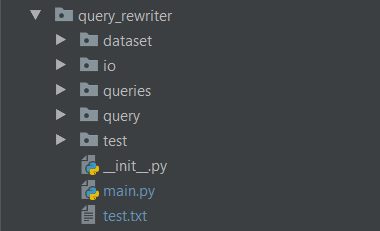
\includegraphics{struct_project.png}
    \caption{Struttura del Progetto}
    \label{fig:struct_project}
\end{figure}

\subsection{Package Dataset}
Il package Dataset include una serie di Dataset in formato csv ed una cartella contente le rispettive liste di RFD già precalcolate. 
I Dataset inclusi nel progetto sono:
\begin{itemize}[noitemsep]
\let\labelitemi\labelitemii
    \item cars.csv
    \item cars2.csv
    \item cars{\_}db.csv
    \item cora.csv
    \item crawled-tweets.csv
    \item dataset.csv
    \item dataset{\_}string.csv
    \item dataset{\_}string2.csv
    \item echocardiogram.csv
    \item iris.csv
    \item restaurant
\end{itemize}

Sono state già calcolate le seguenti liste di RFD:
\begin{itemize}[noitemsep]
\let\labelitemi\labelitemii
    \item cars{\_}db{\_}rfds.csv
    \item cars{\_}rfds.csv
    \item cora{\_}rfds.csv
    \item dataset{\_}rdfs.csv
    \item dataset{\_}strng{\_}rdfs.csv
\end{itemize}


La maggior parte dei Dataset sono in formato numerico, ma ne sono presenti alcuni che possiedono attributi sia in formato numerico che di tipo stringa

\subsection{Package io}
In questo package sono contenuti diversi moduli divisi in baso al loro scopo. Vi sono due sottocartelle che raggruppano il tutto.
Il contenuto nella sottocartela csv comprende:
\begin{itemize}[noitemsep]
\let\labelitemi\labelitemii
    \item csv{\_}parser.py
    \item io.py
\end{itemize}

\paragraph{csv{\_}parser.py}
Questo modulo contiene la classe CSV Parser che si occupa di prendere i dati dai file CSV e salvarli in un dataframe, il tutto viene fatto nel metodo init.
\begin{listing}[H]
\begin{minted}[bgcolor=black,frame=lines,linenos]{python}
class CSVParser:
    def __init__(self, csv_path: str):
        self.path = csv_path
        self.delimiter = self.__guess_delimiter()
        self.data_frame = pd.read_csv(self.path, 
                                delimiter=self.delimiter)
        self.rows_count, self.columns_count = self.data_frame.shape
        self.header = list(self.data_frame)
\end{minted}
\caption{Class CSVParser}
\label{Code:1}
\end{listing}
L'operazione vera e propria di parsing e loading dei dati viene delegata al Framework Pandas, richiamando il metodo alla riga 5
Le variabili di questa classe sono:
\begin{itemize}[noitemsep]
    \item path:[str] Contiene il path del file CSV
    \item delimiter:Contiene il carattere di separazione
    \item data{\_}frame:[Pandas Dataframe] Contiene i dati del file CSV letto
    \item rows{\_}count:[int]contiene il numero di righe contenute nel file CSV
    \item column{\_}count:[int]contiene il numero di colonne contenute nel file CSV
    \item header:[list] contiene una lista di valori che fungono da header, questi valori sono specificati nella prima riga del file csv
\end{itemize}
L'unico argomento da passare al costruttore è il path del file, tutti gli altri dati vengono calcolati. 
All'interno del costruttore è presente una chiamata al metodo {\_\_}guess{\_}delimiter:

\begin{listing}[H]
\begin{minted}[bgcolor=black,frame=lines,linenos]{python}
    def __guess_delimiter(self):
\end{minted}
\caption{Guess delimiter}
\label{Code:2}
\end{listing}

Questo metodo ha il compito di indovinare il carattere di separazione leggendo il file.

\paragraph{io.py}
Questo modulo contiene la classe CSVInputOutput la quale si occupa di importare/esportare una Pandas.Dataframe da/in un file CSV
\begin{listing}[H]
\begin{minted}[bgcolor=black,frame=lines,linenos]{python}
    class CSVInputOutput:
\end{minted}
\caption{CSVInputOutput}
\label{Code:3}
\end{listing}
Le variabili di questa classe sono:
\begin{itemize}[noitemsep]
    \item sep:[str] campo contenente il simbolo di separazione utilizzato nei file CSV
    \item na{\_}rep:[str] campo contenente il simbolo che rappresenta un dato mancante 
    \item index:[boolean] flag che indica se si vuole stampare nel file csv gli indici di riga
    \item encoding:[str] campo contente la codifica dei file input/output
    \item date{\_}format:[str] campo contente il formato delle date
\end{itemize}
Questa classe possiede due metodi.
Il primo è il metodo store
\begin{listing}[H]
\begin{minted}[bgcolor=black,frame=lines,linenos]{python}
    def store(self, df: pd.DataFrame, path: str):
\end{minted}
\caption{store method}
\label{Code:4}
\end{listing}
Questo metodo prende in input il path del del file in cui andare a salvare il DataFrame

Il secondo è il metodo load
\begin{listing}[H]
\begin{minted}[bgcolor=black,frame=lines,linenos]{python}
    def load(self, path: str) -> pd.DataFrame:
\end{minted}
\caption{load method}
\label{Code:5}
\end{listing}
Il metodo prende in input il path del file e delegando a Pandas Dataframe esegue il parsing e il loading


La seconda sottocartella rfd contiene vari moduli inerenti alla manipolazione delle RFD:
\begin{itemize}[noitemsep]
\let\labelitemi\labelitemii
    \item rfd{\_}extractor.py
    \item store{\_}and{\_}load.py
\end{itemize}

\paragraph{rfd{\_}extractor.py}
È contiene la classe RFDExtractor che si occupa di estrarre le RFD da un dataset
rfd{\_}extractor.py
\begin{listing}[H]
\begin{minted}[bgcolor=black,frame=lines,linenos]{python}
class RFDExtractor:
    ...
    def __init__(self, args, debug_mode=False) -> None:
    ...
    def __str__(self) -> str:
    ...
    def extract_args(self, args):
    ...
    def extract_hss(self, cols_count, lhs, rhs):
    ...
    def extract_sep_n_header(self, c_sep, csv_file, has_header):
    ...
    def check_correctness(self, has_dt, hss, index_col):
    ...
    def usage(self):
    ...
    def print_human(self, rfd_data_frame: pd.DataFrame):
    ...
    def get_rfd_dictionary_list(self) -> list:
    ...
\end{minted}
\caption{RFDExtractor}
\label{Code:6}
\end{listing}

Non saranno fornite particolari informazioni su questa classe , in quanto essa fa parte del progetto riguardante la ricerca di RFD , per ulteriori informazioni si veda \cite{tesinaIA}

\paragraph{store{\_}and{\_}load.py}
È un modulo che ha funzione di wrapping per l'algoritmo di ricerca di RFD.
Contiene due metodi:
\begin{listing}[H]
\begin{minted}[bgcolor=black,frame=lines,linenos]{python}
def diff(list1: list, list2: list):
...
def search_rfds(csvPath,name_rfds_file):
\end{minted}
\caption{Metodi store{\_}load{\_}rfds}
\label{Code:7}
\end{listing}

IL primo metodo "diff" prende in input due liste, e restituisce una lista di elementi che sono presenti nella prima ma non nella seconda.

Il secondo metodo richiama l'algoritmo di Ricerca delle RFD \footnote{In questo caso non è semplice richiamo di una funzione, bensì vengono richiamati una serie di metodi, e mano a mano vengono effettuate delle elaborazioni sui dati} e crea un file contente una lista di RFD. Prende in input il path del file contenente il Dataset, e una stringa che contiene il nome del file che incapsula le RFD. 

\subsection{Package query}
Nel package query vi sono tre moduli, tutte e tre si occupano di svolgere operazioni riguardanti le interrogazioni al dataset.
I tre moduli sono:
\begin{itemize}[noitemsep]
\let\labelitemi\labelitemii
    \item query.py
    \item relaxer.py
    \item slicer.py
\end{itemize}

\paragraph{query.py}
Questa classe rappresenta l'oggeto query, ogni condizione della query è rappresentata utilizzato il formato chiave:valore, dove ogni chiave indica l'attributo ed il valore indica il corrispondente valore che stiamo cercando. In parole povere la classe query è una struttura dati\footnote{In python abbiamo ritenuto che la struttura dati migliore fosse quella contenente un dizionario} per immagazzinare la query vera e propria.
Questa classe contiene un metodo
\begin{listing}[H]
\begin{minted}[bgcolor=black,frame=lines,linenos]{python}
def to_expression(self) -> str:
    last_key = list(self.keys())[-1]
    expr = ""
    for k, v in self.items():
        if isinstance(v, range):
            ...
        elif isinstance(v, dict):
            expr += " {} >= {} and {} <= {}".format(k, v['min'],
                                                    k, v['max'])
        elif isinstance(v, (int, float, list)):
            expr += " {} == {}".format(k, v)
        elif isinstance(v, str):
            if "%" in v:
                if v.startswith("%") and v.endswith("%"):
                    expr += k + ".str.contains('{}') ".format(v[1:-1])
                elif v.startswith("%"):
                    expr += k + ".str.endswith('{}') ".format(v[1::])
                elif v.endswith("%"):
                    expr += k + ".str.startswith('{}') ".format(v[:-1])
            else:
                expr += " {} == {}".format(k, v)

        if k is not last_key:
            expr += " and "
    return expr
\end{minted}
\caption{Metodo def{\_}to{\_}express()}
\label{Code:9}
\end{listing}

Questo metodo converte il dizionario nel formato stringa richiesto dal Dataframe di Pandas.
Qui è importante fare delle precisazioni. In questa parte del codice vengono definite le condizioni che si possono applicare alla query.
Nella riga 9 viene implementato la funzionalità di selezione di valori appartenenti ad un range. Possiamo effettuare una query del tipo: \\~\\
\centerline{SELECT * FROM dataset{\_}string WHERE height BETWEEN $value_1$ and $value_2$}
\\~\\
Nella riga 12 viene implementata la funzionalità di uguaglianza per int e float.
Nelle righe dal 13 a 22, viene implementata la funzione di uguaglianza con le stringhe, inoltre è stata implementata anche la funzionalità simil-SQL "LIKE". L'utente può quindi effettuare delle query non solo di uguaglianza, ma anche di contenimento. Ad esempio può chiedere tutte le stringhe che iniziamo per "mary" o che contengono la parola "ohn"


\chapter{Algoritmo Progettato}
In questa sezione saranno illustrati sequenzialmente i passi effettuati dal software. I passi sono  seguenti:
\begin{itemize}[noitemsep]
    \item Caricamento dataset
    \item Caricamento lista RFD
    \item Ordinamento delle RFD
    \item Query Estesa
    \item Query Rilassata
\end{itemize}
\begin{figure}[H]
\centering
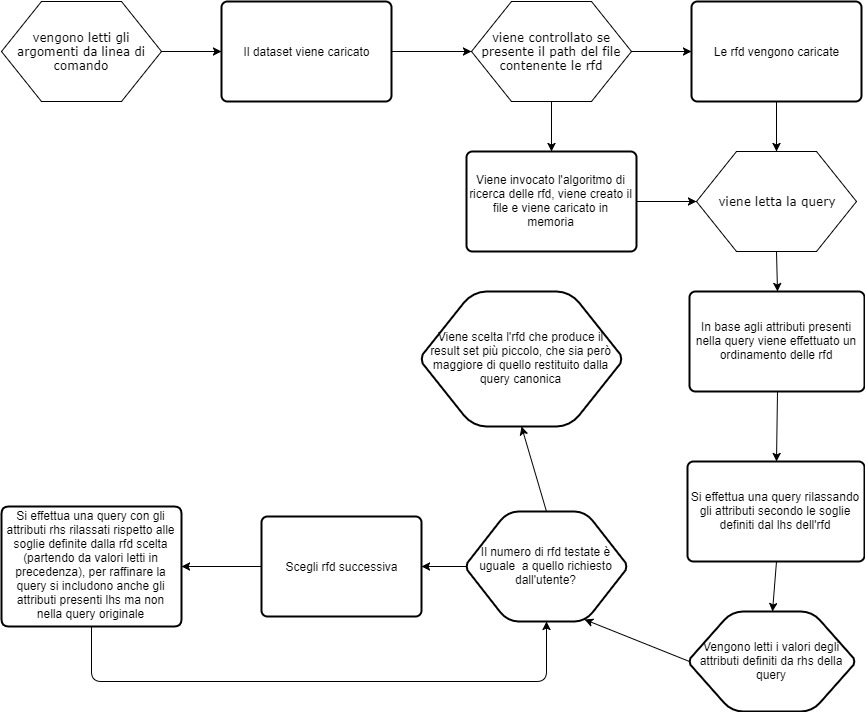
\includegraphics[width=\textwidth,height=\textheight,keepaspectratio]{images/Flowchart.jpg}
\caption{Flowchart}\label{fig:4}
\end{figure}
\paragraph{Caricamento Dataset}
Il primo passo da effettuare è quello di caricare il DataSet in formato csv. Il separatore che di norma può essere costituito da un carattere a scelta è stato impostato come carattere ";".\\ Il DataSet può contenere vari tipi di dati: float, int, stringhe e date.
La struttura dati utilizzata per contenere i dati è quella del pandas.Dataframe , contenuta nel package Pandas\footnote{Pandas è una libreria software scritta per il linguaggio di programmazione Python .È adibita alla manipolazione e l'analisi dei dati. In particolare, offre strutture e operazioni di dati per la manipolazione di tabelle numeriche e di serie temporali. }. \\Il Dataframe di Pandas è una struttura dati tabulare bidimensionale variabile in formato e con assi etichettati (righe e colonne). Le operazioni vengono effettuate sulle righe e sulle colonne. 
\paragraph{Carimento lista RFD}
Il secondo passo consiste nel caricare la lista di RFD. L'utente può passare il path del file contenente le RFD, altrimenti viene invocato un algoritmo di ricerca di RFD sul DataSet indicato.
Nel caso in cui venga passato il path, il formato del file deve essere di tipo csv, con carattere di separazione uguale a ";"\footnote{In realtà è stato implementato un sistema capace di riconoscere ed utilizzare un qualsiasi carattere di separazione}.
Dato che ogni RFD può avere un attributo diverso come parte RHS , si è scelto di utilizzare una particolare notazione:
\begin{table}[H]
    \centering
    \begin{tabular}{l l l l l }
     RHS & $attr_1$ & $attr_2$ & $attr_{\ldots}$ & $attr_n$ \\
    $attr_{k}$ & $s_{12}$ & $s_{13}$ & $s_{\ldots}$ & $s_1n$  \\
    $attr_{j}$ & $s_{22}$ & $s_{23}$  & $s_{\ldots}$ & $s_{2n}$\\
    $attr_{p}$ & $s_{\ldots1}$ & $s_{\ldots3}$  & $s_{\ldots}$ & $attr_{r}$\\
    $s_{m1}$ & $s_{m2}$ & $s_{m3}$ & $s_{\ldots}$ & $s_{mn}$\\
    \end{tabular}
    \caption{Pandas Dataframe contenente le soglie delle RFD}
    \label{tab:RFD_notation}
\end{table}

La prima colonna del Dataframe contiene non una soglia bensì il nome dell'attributo che funge da RHS in quella RFD.
\\
Se l'utente non fornisce il path del file, o se il file non viene trovato, il software richiama l'algoritmo di ricerca delle RFD. Il path del Dataset viene passato all'algoritmo di RFDD\footnote{Relaxed Functional Dependencies Discovery} , dopo aver elaborato restituisce una Dataframe contenente le RFD, le quali vengono salvate su file e successivamente caricate in memoria.
\paragraph{Ordinamento delle RFD}
Una volta caricata la lista di query è necessario effettuare una pulizia sui dati.
Vengono eliminate le RFD che possiedono valore "NaN" su attributi che sono presenti nella query, dopodiché vengono eliminate le RFD dove nel lato RHS è presente un attributo della query \footnote{Utilizzare una RFD di questo tipo significherebbe utilizzare una dipendenza funzionale rilassata banale, la quale non porta alcuna informazione aggiuntiva}
\begin{table}[H]
    \centering
    \begin{tabular}{l l l l l }
     RHS & $attr_1$ & $attr_2$ & $attr_{\ldots}$ & $attr_n$ \\
    $attr_{k}$ & $s_{12}$ & $s_{13}$ & $s_{\ldots}$ & $s_1n$  \\
    $attr_{j}$ & $s_{22}$ & $s_{23}$  & $s_{\ldots}$ & $s_{2n}$\\
    $attr_{p}$ & $s_{\ldots1}$ & $s_{\ldots3}$  & $s_{\ldots}$ & $attr_{r}$\\
    $s_{m1}$ & $s_{m2}$ & $s_{m3}$ & $s_{\ldots}$ & $s_{mn}$\\
    \end{tabular}
    \caption{Pandas Dataframe contenente le soglie delle RFD}
    \label{tab:RFD_notation}
\end{table}
Dopo aver effettuato questa pulizia le RFD vengono ordinate. 
\newline
C'è stata molta indecisione riguardo l'implementazione dell'ordinamento, in quanto non è stata trovata una dimostrazione formale che ci indicasse quale metodo fosse il più efficace.
L'obiettivo è stato quello di trovare un algoritmo che ordinasse le RFD dando precedenza a quelle che producono Result Set non troppo ampi.
\\
Dopo vari test abbiamo pervenuto che il metodo più efficacie fosse quello di ordinare le RFDs prima in ordine decrescente rispetto al numero di attributi con valore "NaN" e poi in ordine crescente di soglia rispetto agli attributi presenti nella query. 
L'ordinare secondo soglie più piccole indica che quelle RFD agiscono su range ridotti, indicativamente ciò significa che rispetto ad un range più ampio un range di dimensioni ridotte include meno dati .In realtà può capitare che in un range di un DataSet vi sia una forte aggregazione di dati , superiore a tutti gli altri dati presenti nel Dataset. Ad esempio preso un Dataset che possiede un attributo altezza possiamo avere i seguenti valori
\begin{table}[H]
    \centering
    \begin{tabular}{l }
    altezza \\
    170 \\
    171 \\
    172 \\
    171 \\
    169 \\
    170 \\
    173 \\
    170 \\
    169 \\
    158 \\
    165 \\
    152 \\
    \end{tabular}
    \caption{Esempio di valori su attributo altezza}
    \label{tab:height_list}
\end{table}
In questo caso se abbiamo due range $[169,172]$ e $[140,165]$, l'intuizione ci dice che il primo range essendo il più piccolo dovrebbe includere meno dati, invece guardando dalla lista si può notare che il primo range contiene 8 valori ed il secondo solo 3.
Ciò capita abbastanza raramente , infatti nei test effettuati questo principio di ordinamento ha restituito quasi sempre i risultati migliori.
Per aumentare l'efficacia dell'ordinamento abbiamo ritenuto necessario dare precedenza alle RFD che nel lato LHS possiedono un numero di attributi il più simile possibile agli attributi presenti nella query.
Nella tabella sottostante viene mostrata parte di una lista di RFD ordinata \footnote{L'ordinamento è stato effettuato in base ad una query eseguita dall'utente, in questo caso la query è SELECT * FROM dataset{\_}string WHERE height=169}:
\begin{table}[H]
    \centering
    \begin{tabular}{l l l l l l l l}
        & RHS & age & height & shoe{\_}size & weight \\
        \hline
    0 & shoe{\_}size & NaN & 0.0 & 1.0 & NaN \\
    1 & weight & NaN & 0.0 & 0.0 & 1.0 \\
    2 & shoe{\_}size & 3.0 & 0.0 & 0.0 & NaN \\
    3 & weight & 6.0 & 1.0 & NaN & 4.0 \\
    4 & weight & NaN & 1.0 & 1.0 & NaN \\
    5 & shoe{\_}size & 6.0 & 1.0 & 1.0 & NaN \\
    6 & shoe{\_}size & NaN & 1.0 & 1.0 & 4.0 \\
    7 & shoe{\_}size & NaN & 1.0 & 0.0 & 2.0 \\
    8 & age & 6.0 & 1.0 & 0.0 & NaN \\
    9 & age & 5.0 & 1.0 & 1.0 & NaN \\
    \ldots & \ldots & \ldots & \ldots & \ldots & \ldots \\
    \end{tabular}
    \caption{Parte di una lista di RFD ordinata}
    \label{tab:ord_rdf}
\end{table}

\paragraph{Query Estesa}
D'ora in poi tutta la procedura descritta da qui in avanti verrà iterata per un numero di RFD pari ad un valore definito dall'utente. \footnote{In caso in cui l'utente lasci il campo vuoto, l'iterazione viene effettuata per ogni RFD presente nella lista}
Viene selezionata la i-esima RFD con $i\in[1,n]$. 
Si vanno a considerare gli attributi della RFD che siano presenti nella query\footnote{In questo momento si considerano solo gli attributi in LHS}, si prendono le soglie e si effettua una nuova una query estesa $Q_2$
Ad esempio supponendo che la query iniziale sia: 
\\~\\ 
\centerline{SELECT * FROM dataset{\_}string WHERE height=169} 
\\~\\
e che la RFD selezionata sia: 
\\~\\ 
\centerline{$(height \leq 0.0)  \rightarrow(shoe_size \leq 0.0)$}
\\~\\
Viene effettuato un controllo sul tipo di valori degli attributi della query,
si vanno a identificare tipi string, int e float, questa identificazione serve a specificare quale funzione di distanza bisogna applicare durante l'estensione della query.
Dato che $height$ è un attributo di tipo numerico, si vanno a prendere tutti i valori che differiscono di 0 dal valore iniziale inserito dall'utente. In questo caso la query estesa $Q_2$ resta uguale a $Q_1$: 
\\~\\
\centerline{SELECT * FROM dataset{\_}string WHERE height =169} 
\\~\\
Effettuando una nuova interrogazione con la query $Q_2$ otteniamo un Result Set che sarà di sicuro $\geq$ del Result Set restituito dall query iniziale.
In questo caso entrambe le query restituiscono questo risultato: \newline 
\begin{table}[H]
    \centering
    \begin{tabular}{l l l l l l l l}
    n.row   & height & weight & shoe{\_}size & age \\
    \hline
    5 & 169 & 73 & 38 & 49 \\
    \end{tabular}
    \caption{Result Set restituito sia dalla query $Q_1$ e sia dalla query $Q_2$ }
    \label{tab:sta_ext_result_set}
\end{table}
\paragraph{Query Rilassata}
In questa procedura viene effettuato il vero e proprio rilassamento, scambiando gli attributi della query con attributi definiti dalla parte RHS della RFD selezionata (vedi Appendice [perfezionamento con lhs]).
Inizialmente si effettua una raccolta dei valori nel dataset, si selezionano solo gli attributi che sono presenti in RHS. Viene mantenuta una struttura dati\footnote{In questo momento lo definiamo come un set} per ogni tupla restituita dal dataset (vedi Appendice [perfezionamento combinazioni]). 
Per ogni Set vengono rilassati i valori in base alle soglie contenute nella RFD, il risultato sarà una serie di SET che contengono dei range più ampi.
È quindi possibile effettuare $k$ query rilassate, ottenendo vari Result Set. La loro unione andrà a costituire il Result Set finale che sarà restituito in output.
Riprendendo l'esempio riportato nel paragrafo precedente, vengono raccolti i dati sui valori presenti in RHS, in questo caso vi è solo l'attributo shoe{\_}sie \footnote{In realtà in RHS vi è sempre un unico attributo, la query viene rilassata con più attributi in quanto si esegue un perfezionamento vedi  Appendice [perfezionamento combinazioni]} che viene rilassato di una soglia pari a 0. Dato che la query estesa $Q_2$ ha restituito una sola tupla, verrà rilassato un unico valore. La query rilassata $Q_3$  è : \newline 
\centerline{SELECT * FROM dataset{\_}string WHERE shoe{\_}size=38}
\newline
Per la proprietà delle RFD (vedi Appendice Proprietà RFD) il Result Set restituito sarà $\geq$ del Result Set restituito dalla query estesa $Q_2$.

In questo caso il Result Set è uguale a :
\begin{table}[H]
    \centering
    \begin{tabular}{l l l l l l l l}
    n.row  & height & weight & shoe{\_}size & age \\
    \hline
    0  & 175 & 75 & 39 & 41 \\
    1  & 169 & 73 & 38 & 49 \\
    2  & 170 & 65 & 39 & 30 \\
    \end{tabular}
    \caption{Result Set restituito sia dalla query $Q_3$ }
    \label{tab:relax_result_set}
\end{table}

Dato che questa procedura viene effettuata per un numero N di RFD, viene effettuato un confronto in modo tale da restituire il Result Set che che sia il meno ampio possibile \footnote{Vengono scartati i Result Set che hanno cardinalità uguale ad Result restituito dalla query iniziale}.




\chapter{Implementazione}
\section{Struttura del Progetto}
Il progetto è incluso in una cartella contenente anche il software di ricerca di RFD, tutto il codice sviluppato è contenuto nella sottocartella query{\_}rewriter
\begin{figure}[H]
    \centering
    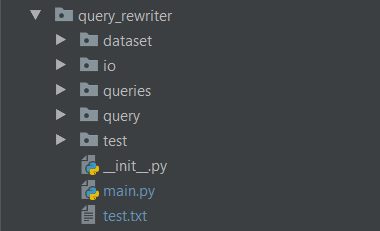
\includegraphics{struct_project.png}
    \caption{Struttura del Progetto}
    \label{fig:struct_project}
\end{figure}

\subsection{Package Dataset}
Il package Dataset include una serie di Dataset in formato $csv$ ed una cartella contente le rispettive liste di RFD già precalcolate. 
I Dataset inclusi nel progetto sono:
\begin{itemize}[noitemsep]
\let\labelitemi\labelitemii
    \item cars.csv
    \item cars2.csv
    \item cars{\_}db.csv
    \item cora.csv
    \item crawled-tweets.csv
    \item dataset.csv
    \item dataset{\_}string.csv
    \item dataset{\_}string2.csv
    \item echocardiogram.csv
    \item iris.csv
    \item restaurant
\end{itemize}

Sono state già calcolate le seguenti liste di RFD:
\begin{itemize}[noitemsep]
\let\labelitemi\labelitemii
    \item cars{\_}db{\_}rfds.csv
    \item cars{\_}rfds.csv
    \item cora{\_}rfds.csv
    \item dataset{\_}rdfs.csv
    \item dataset{\_}strng{\_}rfds.csv
\end{itemize}


La maggior parte dei Dataset sono in formato numerico, ma ne sono presenti alcuni che possiedono attributi sia in formato numerico che di tipo stringa

\subsection{Package io}
In questo package sono contenuti diversi moduli divisi in baso al loro scopo. Vi sono due sottocartelle che raggruppano il tutto.
Il contenuto nella sotto-cartella csv comprende:
\begin{itemize}[noitemsep]
\let\labelitemi\labelitemii
    \item csv{\_}parser.py
    \item io.py
\end{itemize}

\paragraph{csv{\_}parser.py}
Questo modulo contiene la classe CSV Parser che si occupa di prendere i dati dai file CSV e salvarli in un Dataframe, il tutto viene fatto nel metodo init(\ldots).
\begin{listing}[H]
\begin{minted}[frame=lines,linenos]{python}
class CSVParser:
    def __init__(self, csv_path: str):
        self.path = csv_path
        self.delimiter = self.__guess_delimiter()
        self.data_frame = pd.read_csv(self.path, 
                                delimiter=self.delimiter)
        self.rows_count, self.columns_count = self.data_frame.shape
        self.header = list(self.data_frame)
\end{minted}
\caption{Class CSVParser}
\label{Code:1}
\end{listing}
L'operazione vera e propria di $parsing$ e $loading$ dei dati viene delegata al Framework Pandas, richiamando il metodo alla riga 5.
Le variabili di questa classe sono:
\begin{itemize}[noitemsep]
\let\labelitemi\labelitemii
    \item path:[str] Contiene il path del file CSV
    \item delimiter:Contiene il carattere di separazione
    \item data{\_}frame:[Pandas Dataframe] Contiene i dati del file CSV letto
    \item rows{\_}count:[int]contiene il numero di righe contenute nel file CSV
    \item column{\_}count:[int]contiene il numero di colonne contenute nel file CSV
    \item header:[list] contiene una lista di valori che fungono da header, questi valori sono specificati nella prima riga del file csv
\end{itemize}
L'unico argomento da passare al costruttore è il path del file, tutti gli altri dati vengono calcolati. 
All'interno del costruttore è presente una chiamata al metodo {\_\_}guess{\_}delimiter:

\begin{listing}[H]
\begin{minted}[frame=lines,linenos]{python}
    def __guess_delimiter(self):
\end{minted}
\caption{Guess delimiter}
\label{Code:2}
\end{listing}

Questo metodo ha il compito di indovinare il carattere di separazione leggendo il file.

\paragraph{io.py}
Questo modulo contiene la classe CSVInputOutput la quale si occupa di importare/esportare una Pandas.Dataframe da/in un file CSV
\begin{listing}[H]
\begin{minted}[,frame=lines,linenos]{python}
    class CSVInputOutput:
\end{minted}
\caption{CSVInputOutput}
\label{Code:3}
\end{listing}
Le variabili di questa classe sono:
\begin{itemize}[noitemsep]
    \item sep:[str] campo contenente il simbolo di separazione utilizzato nei file CSV.
    \item na{\_}rep:[str] campo contenente il simbolo che rappresenta un dato mancante. 
    \item index:[boolean] flag che indica se si vuole stampare nel file csv gli indici di riga.
    \item encoding:[str] campo contente la codifica dei file input/output.
    \item date{\_}format:[str] campo contente il formato delle date.
\end{itemize}
Questa classe possiede due metodi.
Il primo è il metodo store
\begin{listing}[H]
\begin{minted}[frame=lines,linenos]{python}
    def store(self, df: pd.DataFrame, path: str):
\end{minted}
\caption{store method}
\label{Code:4}
\end{listing}
Questo metodo prende in input il path del del file in cui andare a salvare il DataFrame.

Il secondo è il metodo load:
\begin{listing}[H]
\begin{minted}[frame=lines,linenos]{python}
    def load(self, path: str) -> pd.DataFrame:
\end{minted}
\caption{load method}
\label{Code:5}
\end{listing}
Il metodo prende in input il path del file e delegando a Pandas Dataframe esegue il parsing e il loading.


La seconda sotto-cartella rfd contiene vari moduli inerenti alla manipolazione delle RFD:
\begin{itemize}[noitemsep]
\let\labelitemi\labelitemii
    \item rfd{\_}extractor.py
    \item store{\_}and{\_}load.py
\end{itemize}

\paragraph{rfd{\_}extractor.py}
Contiene la classe RFDExtractor che si occupa di estrarre le RFD da un dataset.
\begin{listing}[H]
\begin{minted}[frame=lines,linenos]{python}
class RFDExtractor:
    ...
    def __init__(self, args, debug_mode=False) -> None:
    ...
    def __str__(self) -> str:
    ...
    def extract_args(self, args):
    ...
    def extract_hss(self, cols_count, lhs, rhs):
    ...
    def extract_sep_n_header(self, c_sep, csv_file, has_header):
    ...
    def check_correctness(self, has_dt, hss, index_col):
    ...
    def usage(self):
    ...
    def print_human(self, rfd_data_frame: pd.DataFrame):
    ...
    def get_rfd_dictionary_list(self) -> list:
    ...
\end{minted}
\caption{RFDExtractor}
\label{Code:6}
\end{listing}

Non saranno fornite particolari informazioni su questa classe , in quanto essa fa parte del progetto riguardante la ricerca di RFD , per ulteriori informazioni si veda \cite{tesinaIA}

\paragraph{store{\_}and{\_}load.py}
È un modulo che ha funzione di wrapping per l'algoritmo di ricerca di RFD.
Contiene due metodi:
\begin{listing}[H]
\begin{minted}[frame=lines,linenos]{python}
def diff(list1: list, list2: list):
...
def search_rfds(csvPath,name_rfds_file):
\end{minted}
\caption{Metodi store{\_}load{\_}rfds}
\label{Code:7}
\end{listing}

IL primo metodo "diff" prende in input due liste, e restituisce una lista di elementi che sono presenti nella prima ma non nella seconda.

Il secondo metodo richiama l'algoritmo di Ricerca delle RFD \footnote{In questo caso non è semplice richiamo di una funzione, bensì vengono richiamati una serie di metodi, e mano a mano vengono effettuate delle elaborazioni sui dati} e crea un file contente una lista di RFD. Prende in input il path del file contenente il Dataset, e una stringa che contiene il nome del file che incapsula le RFD. 

\subsection{Package query}
Nel package query vi sono tre moduli, tutte e tre si occupano di svolgere operazioni riguardanti le interrogazioni al dataset.
I tre moduli sono:
\begin{itemize}[noitemsep]
\let\labelitemi\labelitemii
    \item relaxer.py
    \item slicer.py
\end{itemize}

\paragraph{relaxer.py}
Questo modulo contiene la classe QueryRelaxer, è una classe ausiliaria, contiene dei metodi statici che si occupano di rilassare la query rispetto ad una Relaxed Functional Dependency. La classe contiene i seguenti metodi:

\begin{listing}[H]
\begin{minted}[frame=lines,linenos]{python}
class QueryRelaxer:
    @staticmethod
    def drop_query_nan(rfds_df: pd.DataFrame, query: dict) 
                                            -> pd.DataFrame:
    ...
    @staticmethod
    def drop_query_rhs(rfds_df: pd.DataFrame, query: dict)
                                            -> pd.DataFrame:
    ...
    @staticmethod
    def sort_by_decresing_nan_incresing_threshold(rfds_df: 
                pd.DataFrame, query: dict) -> pd.DataFrame:
    ...
    @staticmethod
    def sort_by_increasing_threshold(rfds_df: pd.DataFrame,
        data_set: pd.DataFrame, query: dict) -> pd.DataFrame:
    ...
    @staticmethod
    def rfd_to_string(rfd: dict) -> str:
    ...
    @staticmethod
    def query_dict_to_expr(query: dict) -> str:
    ...
    @staticmethod
    def extend_query_ranges(query: dict, rfd: dict, 
            data_set: pd.DataFrame = None) -> dict:
    ...
    @staticmethod
    def similar_strings(source: str, data: pd.DataFrame,
                        col: str, threshold: int) -> list:
    ...
    @staticmethod
    def extract_value_lists(df: pd.DataFrame, columns: list):
    ...
\end{minted}
\caption{Classe Query Relaxer}
\label{Code:10}
\end{listing}

Il metodo drop{\_}query{\_}na(...) si occupa di eliminare tutte le RFD che possiedono valori NaN su attributi che sono contenuti anche nella query. Il metodo prende in input un pandas.Dataframe contenente la lista di RFD ed un dizionario contenente la query, restituisce un altro pandas.Dataframe.

Il metodo drop{\_}query{\_}rhs(...) si occupa di eliminare tutte le RFD che possiedono un attributo della query come parte RHS. Il metodo prende in input un pandas.Dataframe contenente la lista di RFD ed un dizionario contenente la query, restituisce un altro pandas.Dataframe.

Il metodo sort{\_}by{\_}decreasing{\_}nan{\_}incresing{\_}threshold(...), contiene un algoritmo di ordinamento. Il metodo prende in input un pandas.Dataframe ordina prima per numero di NaN presenti e poi per ordine crescente rispetto alla soglie, restituisce un pandas.Dataframe.

Il metodo sort{\_}by{\_}increasing{\_}threshold(...) , contiene un altro algoritmo di ordinamento, che è stato utilizzato solo nei test, dove è risultato poco producente. Il metodo prende in input un pandas.Dataframe e un dizionario contenente la query. Restitusce un altro pandas.Dataframe ordinato solo rispetto alle soglie degli attributi \footnote{In entrambi gli algoritmi di ordinamento vengono ordinate prima le soglie degli attributi contenuti nella query e poi in caso di valori uguali si ordina rispetto alle soglie degli altri attributi in LHS}.

il metodo rfd{\_}to{\_}string(...) svolge un ruolo alquanto semplice, si occupa di convertire il formato delle RFD in un formato stringa facilmente leggibile.

Questo metodo converte il dizionario nel formato stringa richiesto dal Dataframe di Pandas.
Qui è importante fare delle precisazioni dato che in  questa parte del codice vengono definite le condizioni che si possono applicare alla query.
Nella riga 9 viene implementato la funzionalità di selezione di valori appartenenti ad un range. Possiamo effettuare una query del tipo:
\\~\\
\centerline{SELECT * FROM dataset{\_}string WHERE height BETWEEN $value_1$ and $value_2$}
\\~\\
Nella riga 12 viene implementata la funzionalità di uguaglianza per int e float.
Nelle righe dal 13 a 22, viene implementata la funzione di uguaglianza con le stringhe, inoltre è stata implementata anche la funzionalità simil-SQL "LIKE". L'utente può quindi effettuare delle query non solo di uguaglianza, ma anche di contenimento. Ad esempio può chiedere tutte le stringhe che iniziamo per "mary" o che contengono la parola "ohn".

\begin{listing}[H]
\begin{minted}[frame=lines,linenos]{python}
def to_expression(self) -> str:
    last_key = list(self.keys())[-1]
    expr = ""
    for k, v in self.items():
        if isinstance(v, range):
            ...
        elif isinstance(v, dict):
            expr += " {} >= {} and {} <= {}".format(k, v['min'],
                                                    k, v['max'])
        elif isinstance(v, (int, float, list)):
            expr += " {} == {}".format(k, v)
        elif isinstance(v, str):
            if "%" in v:
                if v.startswith("%") and v.endswith("%"):
                    expr += k + ".str.contains('{}') ".format(v[1:-1])
                elif v.startswith("%"):
                    expr += k + ".str.endswith('{}') ".format(v[1::])
                elif v.endswith("%"):
                    expr += k + ".str.startswith('{}') ".format(v[:-1])
            else:
                expr += " {} == {}".format(k, v)

        if k is not last_key:
            expr += " and "
    return expr
\end{minted}
\caption{Metodo def{\_}to{\_}express()}
\label{Code:9}
\end{listing}

Il metodo extend{\_}query{\_}ranges(...) prende in input una query ed una RFD ed estende i range sugli attributi basandosi sulle soglie contenute nella RDF. Nel caso in qualche attributo della query è di tipo stringa vengono calcolate le stringhe simili e vengono utilizzare nella query estesa.

Il metodo similar{\_}string() prende in input una stringa, una pandas.Dataframe ed una soglia e si occupa di trovare nel database tutte le stringhe che differiscono di una soglia $\epsilon$. Restituisce un altro pandas.Dataframe.

Il metodo extraxt{\_}value{\_}list(...) prende in input un pandas.Dataframe ed una lista contenente le colonne di cui si vogliono estrarre i valori. Questo metodo restituisce un dizionario di liste, ognuna delle quali ha come chiave il nome dell'attributo.

\paragraph{slicer.py}
È una classe ausiliaria che contiene un solo metodo.
\begin{listing}[H]
\begin{minted}[frame=lines,linenos]{python}
class Slicer:
    @staticmethod
    def slice(df: pd.DataFrame) -> list:
\end{minted}
\caption{Metodo def{\_}to{\_}express()}
\label{Code:14}
\end{listing}

Il metodo slice() si occupa di dividere un pandas.Dataframe, ogni tupla andrà a formare un nuovo Dataframe, viene restituita una lista di DataFrame.

\subsection{Modulo main.py}
Modulo che lancia il programma vero e proprio. Richiede
l'inserimento del nome di un Dataset, assieme ad una serie di opzioni
facoltative, secondo la seguente struttura:
\begin{listing}[H]
\begin{minted}[frame=lines,linenos]{python}
python main .py -p <path-of-dataset > -q <query> [ options ]
\end{minted}
\end{listing}

dove:
\begin{itemize}
\item path-of-dataset è il path relativo Dataset da utilizzare per le query.
\item query è il parametro contenente la query, essa può avere la seguente struttura\footnote{I valori nel caso siano in formato stringa vanno racchiusi fra apici singoli. Ciò viene fatto per evitare problemi nella lettura di eventuali spazi bianchi.}:
\begin{itemize}
\item query semplice : \mint{json}|"{'nome_attributo',valore_attributo}"|
\item query con funzione like : \mint{json}|"{'nome_attributo','%value%'}"|
\item query con controllo su range :  \mint{json}|"{'nome_attributo',{'min':min_val,'max':max_val}}"|
\end{itemize}
\end{itemize}
e [options] può contenere zero o più delle seguenti opzioni:

\begin{itemize}
\item -r $<$rfds-path$>$ : nome del file in cui sono salvate le RFD, se non viene fornito le RFD vengono calcolate.
\item -n $<$number-of-test$>$ : numero di RFD da testare, se non viene fornito il test viene effettuato per tutte le RFD contenute nella lista.
\item -o $<$path-output$>$ : nome del file in cui salvare l'output del processo di Query Relaxing.
\end{itemize}


\paragraph{Metodo main()}
Il metodo main() è il primo metodo ad essere eseguito di occupa di leggere e controllare alcuni parametri passati da linea di comando. Una volta processati esso richiama il metodo start{\_}process().

\paragraph{Metodo start{\_}process()}
Questo metodo rappresenta il core del software, incapsula tutti i processi di Query Relaxation.
Segue ora una lista dei metodi che vengono richiamati:
\begin{enumerate}
    \item Inizialmente si occupa di leggere il DataSet richiamando i metodi della classe CSVInputOutput.
    \item Viene effettuato il caricamento della lista di RFD, se tale file non esiste viene generato,
    \item Viene effettuato un cleaning del DataFrame contenente le RFD, dopodiché viene ordinato.
    \item Per ogni RFD i contenuta nella lista \footnote{Vi è un parametro per specificare il numero massimo di RFD da testare} si itera nel seguente modo :
    \begin{itemize}
        \item Si effettua una query estesa rispetto alle soglie della RFD i-esima.
        \item Vengono caricati ,dal Result Set ,tutti i valori degli attributi che sono nella parte RHS della query, inoltre vengono caricati anche i valori degli attributi LHS che non sono nella query. Viene mantenuto un DataFrame per ogni tupla risultante nel Result Set.
        \item Tutti i valori nei DataFrame generati precedentemente vengono estesi rispetto alla soglie della RFD i-esima.
        \item Viene effettuata una query unendo (con degli or) tutte le condizioni contenute nel DataFrame.
        \item Il Result Set contenuto dalla query rilassata viene salvato in memoria.
    \end{itemize}
    \item Viene restituito in output il Result Set meno ampio possibile, che sia però di cardinalità maggiore a quello restituito dalla query originale. Il Result set viene automaticamente salvato in un file formato JSON.
\end{enumerate}


\section{Installazione}
\paragraph{Requisiti}
La versione di Python utilizzata è la 3.6.2 , è stata utilizzati su di un architettura a x64.
Dato che buona parte del codice richiama metodi scritti in Cython , serve un compilatore C++. È stato utilizzato un compilatore della Microsoft incluso nel pacchetto Visual Studio Community 2017 \\
Il progetto contiene le seguenti dipendenze:
\begin{itemize}[noitemsep]
\item[-] click $\geq$ 6.7
\item[-] Cython $\geq$ 0.25.2
\item[-] Flask $\geq$ 0.12.2
\item[-] itsdangerous $\geq$ 0.24
\item[-] Jinja2 $\geq$ 2.9.6
\item[-] MarkupSafe $\geq$ 0.23
\item[-] matplotlib $\geq$ 2.0.2
\item[-] nltk $\geq$ 3.2.4
\item[-] numpy $\geq$ 1.13.0
\item[-] pandas $\geq$ 0.19.2
\item[-] pyparsing $\geq$ 2.2.0
\item[-] python-dateutil $\geq$ 2.6.0
\item[-] pytz $\geq$ 2017.2
\item[-] six $\geq$ 1.10.0
\item[-] tornado $\geq$ 4.5.1
\item[-] Werkzeug $\geq$ 0.12.2
\item[-] editdistance $\geq$ 0.3.1
\item[-] cycler $\geq$ 0.10.1
\item[-] pip $\geq$ 9.0.1
\item[-] setuptools $\geq$ 36.5.0
\item[-] rfd-discovery $\geq$ 0.0.1
\end{itemize}
\paragraph{Installazione}

\begin{enumerate}
\item Scaricare Python (link: https://www.python.org/downloads/release/python-362/), fare attenzione a scegliere la versione in base all'architettura della macchina su cui verrà eseguito il software.
\item Scaricare ed installare il pacchetto "Sviluppo applicazioni desktop con C++" ottenibile da Visual Studio Community 2017 (link: https://www.visualstudio.com/it/thank-you-downloading-visual-studio/?sku=Community\&rel=15)
\item Aggiugere alla variabile di ambiente PATH i seguenti valori:\\ "D:\textbackslash Programmi\textbackslash VS\textbackslash VC\textbackslash Tools\textbackslash MSVC\textbackslash 14.11.25503\textbackslash bin\textbackslash HostX64\textbackslash x64"\\
"C:\textbackslash Program Files (x86)\textbackslash Windows Kits\textbackslash 10\textbackslash bin\textbackslash x64"\footnote{La posizione di tali cartelle può variare}
\item Aprire il "Prompt dei comandi degli strumenti nativi x64(o x86 per sistemi a 32 bit) per VS 2017" ed eseguire il comando "python -m pip install -U pip setuptools"
\item Scaricare il progetto (link: https://github.com/izio7/AttributedGraphProfiler)
\item Spostarsi all'interno della Root del progetto ed aprire il terminale.
\item Eseguire il comando "virtualenv venv" per creare un Virtual Environment in cui eseguire il progetto
\item Eseguire il comando "venv\textbackslash Scripts \textbackslash activate" con cui si si accede al Virtual Environment \footnote{Sotto ambiene Linux\textbackslash MacOS il comando da eseguire è "source venv/bin/activate"}
\item Eseguire il comando "pip install -r requirements.txt" per installare le dipendenze richieste.\footnote{Se si esegue il software in un ambiente di sviluppo dedicato questa operazione viene effettuata automaticamente}
\item Eseguire il comando "python setup.py install"
\item Eseguire i comando "python build.py build{\_}ext --inplace" per effettuare generare il codice C tramite Cython
\item Ora il software è pronto per eseguire le Query rilassate, il main si trova all'interno della folder "query{\_}rewriter"
\end{enumerate}


\chapter{Conclusioni}
\section{Test}
Durante il lavoro di tesi sono stati svolti alcuni test. 
Sono stati eseguiti su una macchina con sistema operativo Windows 10, un processore Intel Core i7 6700HQ a 2.60GHz (6M Cache, up to 3.50 GHz) e con 16Gb di RAM DDR4.

Si possono evidenziare tre gruppi:
\begin{itemize}
    \item Test per il \textit{Reverse Engineering}
    \item Test di integrità 
    \item Test di prestazione
\end{itemize}

\subsection{Test di Reverse Engineering}
Il progetto riguardante la ricerca di dipendenze funzionali rilassate non possedeva una documentazione esaustiva. Per tale motivo si è deciso di creare delle classi Test, che avessero il compito di mostrare il processo effettuato da ogni modulo.
Le classe di test create sono:
\begin{itemize}[noitemsep]
\let\labelitemi\labelitemii
    \item diff{\_}test.py : utilizzata per comprendere il funzionamento della classe che genera la matrice delle differenze.
    \item relaxer{\_}test.py: utilizzata per testare la classe QueryRelaxer.
    \item rfd{\_}extractor{\_}test.py utilizzata per testare il modulo che funge da Bridge per l'algoritmo di ricerca di RFD.
\end{itemize}

\subsection{Test di integrità}
Durante lo sviluppo sono state create delle classi per il testing. Seppur non paragonabili a dei test di unità sono state utili per controllare il funzionamento di ogni singolo modulo.
\begin{itemize}[noitemsep]
\let\labelitemi\labelitemii
    \item io{\_}test.py: utilizzata per testare la classe RFDInputOutput().
    \item csv{\_}parser{\_}test.py : utilizzata per controllare il corretto funzionamento della classe CSVParser. 
    \item csv{\_}test.py: utilizzata per controllare la corretta estrazione dell'header.
    \item dataframe{\_}row{\_}slicer{\_}test.py : utilizzata per controllare il corretto funzionamento della classe Slicer.
    \item similar{\_}strings{\_}test.py utilizzata per testare la funzionalità di ricerca di stringhe simili.
\end{itemize}
\subsection{Test di prestazione}
Per misurare le prestazioni non è stato creato un modulo ad hoc, bensì sono stati eseguiti due gruppi di test manuali:
Il primo gruppo di test è servito a testare la bontà dell'ordinamento delle RFD. 
Un buon ordinamento di RFD deve porre prima le RFD che ampliano il Result Set di poco,
in modo tale da evitare di produrre un Result Set che contengano dati poco inerenti all'interrogazione iniziale.
Per effettuare questo controllo sono stati dichiarate tre variabili:
\begin{itemize}
    \item original{\_}query{\_}result{\_}set{\_}size : una variabile che contiene la cardinalità del Result Set restituito inzialmente.
    \item relaxed{\_}query{\_}result{\_}set{\_}size : una variabile che contiene la cardinalità del Result Set restituito dalla query rilassata.
    \item dataset{\_}size : una variabile che contiene la cardinalità del Dataset
\end{itemize}



Si è deciso di applicare un ottimizzazione sulla ricerca dell'RFD migliore. 
Ogni volta che viene effettuata una Query Rilassata, prima restituire il Result Set, vengono testate le prime N RFD.
Grazie a questi variabili è possibile controllare quanto aumenta la cardinalità del Result Set per ogni RFD. Viene quindi restituita l'RFD che produce il Result Set meno ampio possibile che sia però maggiore del Result Set restituito dalla query iniziale. In questo modo si cercano di ottenere i risultati che siano maggiormente correlati con l'interrogazione iniziale.

Il secondo gruppo di test è stato eseguito verificare quanto tempo chiedesse l'algoritmo.
Si deciso di non tener conto dei tempi di ricerca/caricamento delle RFD, in quanto non dipendendo direttamente dal lavoro sviluppato.

\begin{figure}
    \centering
    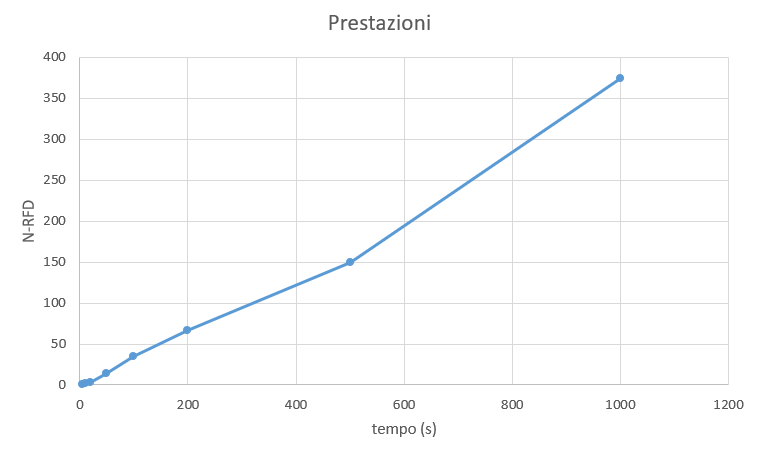
\includegraphics{Prestazioni.PNG}
    \caption{Prestazioni}
    \label{fig:prestazioni}
\end{figure}

\section{Riflessioni}
Dopo aver completato la descrizione del progetto sviluppato è necessario fare qualche osservazione.
L'idea iniziale non è era quella di sviluppare un modulo professionale che permetta il rilassamento di query, bensì lo scopo principale è stato quello di dimostrare che è possibile creare un sistema di rilassamento basato sulle RFD.

Il sistema , seppur necessitando di diverse migliorie, è stato sviluppato in modo da essere facilmente manutenibile. 
Si può collegare facilmente il modulo ad un sistema di ricerca su Web, l'unica limitazione è data dalla poca scelta di comandi SQL, che sono però facilmente modificabili.
Il progetto ha richiesto circa 2 mesi sviluppo per essere completato. Si è svolto sotto la supervisione del prof. Vincenzo Deufemia e della dott.ssa Loredana Caruccio. Il si è svolto con il collega Maurizio Casciano.

\section{Lavori futuri}
Seguono ora alcuni idee da implementare in futuro.
\paragraph{Preferenze utente}
Qualsiasi ordinamento di RFD che non tiene conto del grado di importanza degli attributi per l'utente, difficilmente produrrà un sistema che sia in grado di dare il risultato cercato.
Il problema consiste nell'impossibilità di verificare tutti i possibili legami che esistono all'interno di un Database, ed anche \footnote{Un in Universo in cui ciò sia fattabile} analizzandole tutte, non è detto che l'RFD scelta restituira il risultato cercato dall'utente. Perchè cio?
Il problema sta nell'andare a capire su cosa l'utente è disposto a cedere. Se inizialmente effettua una query contente tre attributi, l'utente magari su alcuni di essi è disposto ad essere flessibile, mentre su altri non vuole compromessi \footnote{Si pensi a quando si cerca un prodotto su di uno Store, quasi nessuno vuole compromessi sul parametro "prezzo"}.
Si suggerisci quindi di implementare un sistema che permetta all'utente di specificare il grado di flessibilità di ogni parametro.
\paragraph{Sistema di query SimilSQL}
Le attuali opzioni di query sono abbastanza scarne, è consigliabile implementare ulteriori opzioni, prendendo d'esempio quelle del SQL. In particolare servirebbero le opzioni: groupby,orderby,in,join.
Tranne la "join" che richiede una revisione della struttura del progetto, il resto è facilmenete implementabile.
\paragraph{Parallelizzazione}
Tutto il progetto è stato sviluppato senza parallelizzazione. Sia l'ordinamento che la scelta della query rilassata è facilmente parallelizzabile. Ciò può portare ad un aumento delle prestazioni, di conseguenza diventa più semplice effettuare maggiori test sulle RFD, permettendo cosi di ottenere Result Set che siano di maggior interesse per l'utente.

\bibliographystyle{plain}
\bibliography{references}
\end{document}
